\chapter{Unsupervised Approach}
Autoencoder wirn 2017 +
Qua veine presentato  il metodo solo OCSVM 

intro sui novelty e loro utilità/vantaggi ( ledebolezze el mettiamo nel chaper 6: copiare da siamesi)


\section{Novelty detection algorithm for human fall detection based on One-Class Support Vector Machine}


The approach proposed in this section is based on a One-Class Support Vector Machine (OCSVM) \cite{scholkopf2000} to obtain an unsupervised framework for Fall Detection.
The acoustic signals are captured by means the Floor Acoustic Sensor and then MFCCs and Gaussian Mean Supervectors (GMSs) are extracted by using the same methods described in \secref{sec:svm_multi_classification}: GMSs are higher level features computed by adapting the means of a Gaussian mixture model (GMM) with maximum a posteriori algorithm (MAP).
In the training phase, a large set of audio data is used to model an Universal Background Model (UBM) composed of the GMM extracted by using Expectation Maximization (EM) algorithm \cite{bilmes1998gentle}.
Then, the GMS of each event is calculated by adapting the GMM with the MAP algorithm and concatenating the resulting GMM mean values.
Abnormal acoustic events are discriminate from normal ones employing the OCSVM classifier.
The performance of the algorithm has been evaluated on a corpus containing sounds of human falls, falling objects, human activities, and music.

\subsection{Dataset}
The performance of the algorithm has been evaluated on a corpus containing sounds of human falls, falling objects, human activities, and music. In particular, from the dataset presented in \secref{sec:dataset}, have been used the samples reported in \tableref{tab:ocsvm_dataset}.

\begin{table}[t]
	\caption{Composition  of the dataset.}
	\label{tab:ocsvm_dataset}
	\begin{center}
		\begin{tabular}[t]{c>{\centering}m{5cm}c}
			
			\hline
			\textbf{Class} & \textbf{Nr. of occurrences} & \textbf{Total length (s)} \\ %\cline{2-5} 
			%& \hspace{8pt}Clean\hspace{8pt}  & \hspace{6pt}Clean\hspace{6pt}   \\ 
			\hline
			Basket      			& 64    &   86    \\
			Fork        			& 64    &   82     \\
			Ball       			& 64    &   129     \\
			Book        			& 64    &   63    \\
			Bag         			& 64    &   57     \\
			Chair       			& 96    &   157     \\
			$\,$ Human Falls $\,$ 	& 44    &   76     \\
			Human Activity  		& 665   &   1218     \\
			Music					& 776   &	1498	\\
			%				 Classic Music       	& 441   &   882     \\
			%				 Rock Music       		& 335   &   616     \\
			\hline
		\end{tabular}
	\end{center}
\end{table}

Musical tracks and normal activities sounds have been divided in segments whose lengths have mean and standard deviation estimated from instances of fall events. In addition, they have been employed alone and to create noisy versions of human and object falls occurrences in order to assess the algorithm in presence of interferences.

In the experiments, signals have been downsampled to 8\,kHz and the resolution has been reduced to 16\,bit. As in the approach presented previously, the choice of the sampling frequency is motivated by the analysis performed in a previous work by the authors \secref{ssec:sig_analysis}, where it was shown that the signals recorded with the FAS have the majority of the energy concentrated at frequencies below 1\,kHz.

\subsection{Experimental setup}

The dataset described previously has been divided in one set for training the UBM and the OCSVM and three sets for evaluating the performance.

Training has been performed on the set shown in \tableref{tab:trainComposition} composed of 947 occurrences (1773\,s) of human activities, classical music and rock music. The assessment of the algorithm has been performed on the following datasets:
\begin{itemize}
	\item Set 1 (Human fall and background sounds): this set comprises 44 examples of human fall sounds and 44 examples of human activity and music sounds (\tableref{tab:set1Composition}).
	\item Set 2 (Human fall and object fall sounds): this set comprises 44 examples of human fall sounds and 44 examples of object fall sounds (\tableref{tab:set2Composition}).
	\item Set 3 (Human fall, object fall and background sounds): this set comprises 44 examples of human fall sounds, 22 examples of background sounds and 22 examples of object fall sounds (\tableref{tab:set3Composition}).
\end{itemize}



\begin{table}[t]
	\caption{Composition  of the training-set.}
	\label{tab:trainComposition}
	\begin{center}
		\begin{tabular}{c>{\centering}m{5cm}c}			
			\hline
			\textbf{Class} & \textbf{Nr.\ of occurrences}  & \textbf{Total length (s)} \\ 
			\hline
			Human Activity  		& 320 &  593		\\
			Music					& 627 &  1180       \\
			%			 Classic Music       	& 306 &  591		\\
			%			 Rock Music       		& 321 &  589 	 	\\
			\hline
			Total                 & 947 & 1773 \\
			\hline
		\end{tabular}		
	\end{center}
\end{table}

\begin{table}[t]
	\centering

	\caption{Composition  of ``Set 1''.}
	\label{tab:set1Composition}
	\begin{center}
		\begin{tabular}{K{3cm}K{3cm}}				
			\hline
			\textbf{Class} & \textbf{Nr.\ of occurrences} \\ 
			\hline
			$\,$ Human Falls $\,$ 	& 44    			\\
			Human Activity  		& 15		\\
			Music			  		& 29		\\
			%				 Classic Music       	& 15   		\\
			%				 Rock Music       		& 14  		\\		
			\hline
		\end{tabular}			
	\end{center}		


	
\end{table}

\begin{table}[t]
	\centering
		
	\caption{Composition  of ``Set 2''.}
	\label{tab:set2Composition}
	\begin{center}
		
		\begin{tabular}{K{3cm}K{3cm}}
			
			\hline
			\textbf{Class} & \textbf{Nr. of occurrences} \\ 
			%& \hspace{8pt}Clean\hspace{8pt}  & \hspace{6pt}Clean\hspace{6pt}   \\ 
			\hline
			$\,$ Human Falls $\,$ 	& 44    		\\				
			Basket      			& 7           	 \\
			Fork        			& 7           	 \\
			Ball       			& 8           	 \\
			Book        			& 7          	  \\
			Bag         			& 8          	  \\
			Chair       			& 7    			\\
			
			\hline
		\end{tabular}
		
	\end{center}
	
\end{table}


\begin{table}[t]
	
	\caption{Composition  of ``Set 3''.}
	\label{tab:set3Composition}
	\begin{center}
		
		\begin{tabular}{K{3cm}K{3cm}}
			
			\hline
			\textbf{Class} & \textbf{Nr. of occurrences} \\ 

			\hline
			$\,$ Human Falls $\,$ 	& 44    		\\				
			Basket      			& 3            	\\
			Fork        			& 4            	\\
			Ball       			& 4            	\\
			Book        			& 3            	\\
			Bag         			& 4            	\\
			Chair       			& 4    			\\
			Human Activity  		& 8   			\\
			Music			  		& 14   			\\
			%				 Classic Music       	& 7   			\\
			%				 Rock Music       		& 7   			\\
			
			\hline
		\end{tabular}
		
	\end{center}
		
\end{table}

For each set, the data have been divided in four folds, each composed of 11 human falls and 11 non-falls. Then, one fold has been used for estimating the hyperparameters of the algorithm and three for calculating the performance. The final performance is calculated by using the cumulative true positives, false positives, and false negatives obtained by varying the test folds.
The validation phase consisted in searching for the number of components of the UBM, the values of $\nu$ and $\gamma$ of the OCSVM. The values assumed by these variables are summarised in \tableref{tab:parameter}.

\begin{table}[t]
	\centering
	\caption{Hyperparameters of the algorithm and search space explored in the validation phase.}
	\label{tab:parameter}
	\begin{tabular}{c |c | c}
		\hline
		\textbf{Stage} & \textbf{Hyperparameter} & \textbf{Range} \\
		\hline
		UBM & $J$ & $1, 2, 4, \ldots , 64$\\
		\hline
		\multirow{2}{*}{OCSVM} & $\nu$ & $0.1, 02, \ldots, 1.0$ \\
		&$\gamma$ & $2^{-15}, 2^{-13}, \ldots,2^{3} $ \\
		\hline

	\end{tabular}
\end{table}


The proposed approach has been compared to the algorithm presented in \cite{Popescu2009} based on OCSVM. The same algorithm has also been employed in \cite{SalmanKhan2015} with a multi-microphone acquisition setup and a source separation stage. As in \cite{Popescu2009}, the audio signals are divided in windows of the same lengths, and the related MFCCs are used for training the OCSVM and for classification. In \cite{Popescu2009}, 7 MFCCs were extracted from audio signals sampled at 20\,kHz and the length of the window was set to 1\,s. Here, the feature vectors are the same of the proposed approach, i.e., they are composed of the first 13 MFCCs and their first and second derivatives. The same window length of \cite{Popescu2009} cannot be employed here, since the dataset used in this paper comprises signals with lengths less than 1\,s. Thus, the length of the window corresponds to the duration of the shortest event in the dataset, and it is equal to 576\,ms (71 frames). Windows are overlapped by 50\%, and, as in \cite{Popescu2009}, an event is classified as fall if at least two consecutive frames are classified as novelty by the OCSVM. The same grid search procedure of the proposed approach has been adopted to search for the optimal values of $\nu$ and $\gamma$ of the OCSVM.


The performance has been evaluated in terms of F$_1$-Measure calculated as:
\begin{equation}
\text{F}_1\text{-Measure} = \frac{2\cdot tp}{2\cdot tp+fn+fp},
\end{equation}
where $tp$ is the number of correctly classified falls, $fn$ is the number of falls misclassified as non-falls, and $fp$ is the number of non-falls misclassified as falls.


\subsubsection{Results and discussion}
\figref{fig:res_clean} shows the results in clean conditions obtained with the proposed method named ``OCSVM'' and the comparative method proposed in \cite{Popescu2009} denoted as ``Popescu (2009)''. Observing the figure, it is evident that in all the three cases the OCSVM approach is able to improve the performance with respect to ``Popescu (2009)'' \cite{Popescu2009}. In particular, in ``Set 1'', that comprises human falls, human activities and music, the performance improves by 16.73\% with respect to ``Popescu (2009)''. This case can be considered as the least challenging of the three, since non-falls events are considerably different from falls ones. Conversely, ``Set 2'' comprises both human falls and object falls, thus it includes abnormal events whose pattern is similar to the one of human falls. Indeed, the performance with respect to ``Set 1'' is 17.91\% lower, mostly due the increased false positives rate that goes from 13.64\% to 50.76\%. Regarding ``Popescu (2009)'' \cite{Popescu2009}, the F$_1$-Measure is below both OCSVM and the proposed approach, however it is less affected by the presence of object falls, since the F$_1$-Measure decreases only by 0.64\% . ``Set 3'' comprises human falls, human activities, music and object falls and represents the most realistic test condition of the three. The results obtained by using  the OCSVM classifier alone is 82.25\%. As expected, this result is lower than ``Set 1'', since object falls are also present, and higher than ``Set 2'', since human activities and music segments are easier to discriminate.  Differently, the approach by Popescu and Mahnot \cite{Popescu2009} degrades by 5.25\% with respect to ``Set 1'', and by 4.61\% with respect to ``Set 2'', demonstrating that it is less robust to the concurrent presence of object falls and daily human activities sounds. 

\begin{figure}[t]
	\centering
	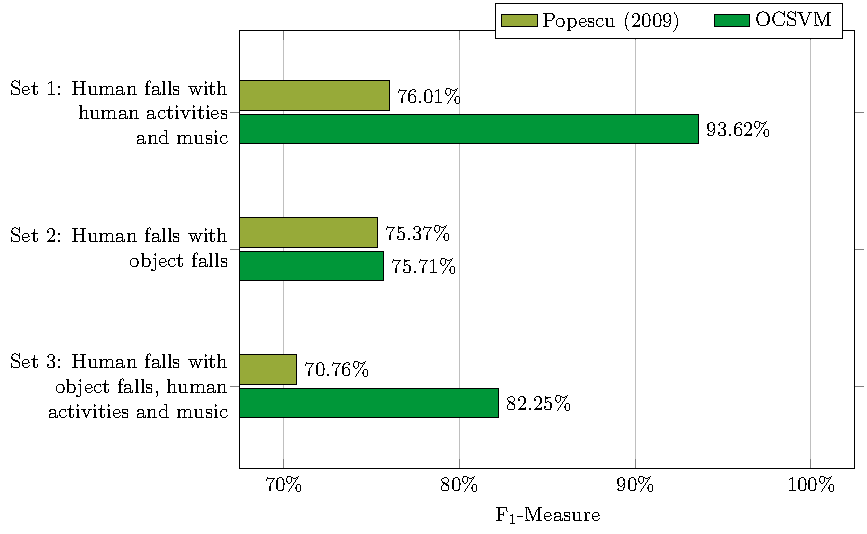
\includegraphics[width=\columnwidth]{img/cin_only_ocsv/res_clean.pdf}
	\caption{Results in \textit{clean} conditions for the three test cases. ``Set 1'' comprises human falls, human activities and music. ``Set 2'' comprises human falls and object falls. ``Set 3'' comprises human falls, object falls, human activities, and music.} \label{fig:res_clean}
\end{figure}

\figref{fig:res_noisy} shows the results obtained for the three cases in noisy conditions. As expected, the performance decreases in all the two evaluated methods. In ``Set 1'', the performance decrease is modest (2.32\% for the OCSVM and 1.44\% for ``Popescu (2009)''), demonstrating that the OCSVM is able to effectively reject non-fall events corrupted by music interference. In ``Set 2'', the presence object falls corrupted by music significantly decreases the performance of the OCSVM, reducing the F$_1$-Measure by 12.74\% with respect to the clean ``Set 2''. The method by Popescu and Mahnot \cite{Popescu2009} achieves the highest F$_1$-Measure in this case, confirming the good capabilities of rejecting dropping objects sound events observed in clean conditions. In ``Set 3'', the proposed approach improves the performance by 3.91\% with respect to ``Popescu (2009)'', confirming that it is able to achieve the highest performance in the most realistic scenario of the three.


\begin{figure}[t]
	\centering
	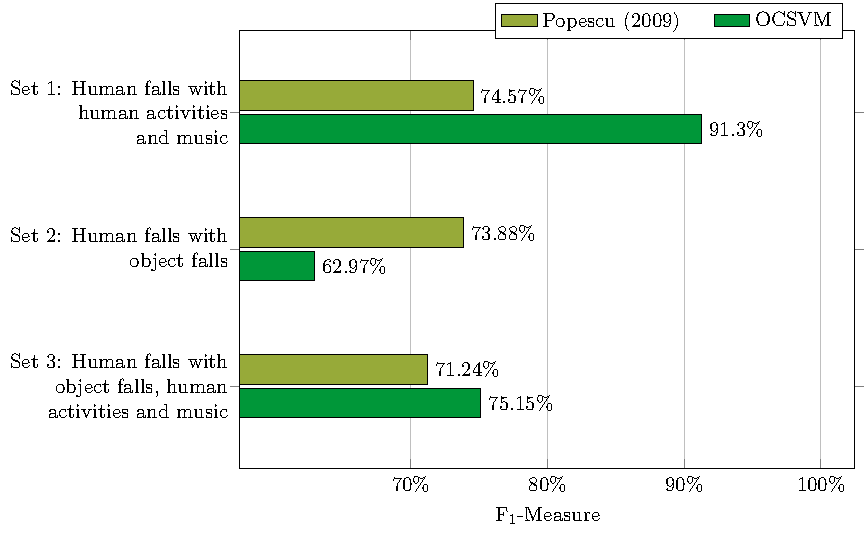
\includegraphics[width=\columnwidth]{img/cin_only_ocsv/res_noisy.pdf}
	\caption{Results in noisy conditions for the three test cases. ``Set 1'' comprises human falls, human activities and music. ``Set 2'' comprises human falls and object falls. ``Set 3'' comprises human falls, object falls, human activities, and music.} \label{fig:res_noisy}
\end{figure}




%\label{sec:ocsvm}}
\section{End-To-End Unsupervised Approach employing Convolutional Neural Network
Autoencoders for Human Fall Detection} CONTROLLA GRAFIOCO RISULTATO ERRORE FORSE!
\label{sec:autoencoder}

The ``analytical methods'' distinguish between fall and non-fall events by applying a threshold directly on the acquired signals or on the features sequences extracted from them \cite{noury2007fall}.
These methods are generally built exploiting some a-priori knowledge to operate in a specific scenario and needs manual tuning of the hyperparameters of the algorithm. For these reasons, the ``analytical methods'' can hardly perform when the operating conditions and the subjects are variable. In ``machine learning'' methods, the algorithm learn from the data how to discriminate falls from non-falls \cite{noury2007fall}. Between them can be distinguished ``supervised'' and  ``unsupervised'' approaches. The fist  require a labelled dataset for training the classifier, while the latter build a normality model considering only the non-fall events. Regardless of the used approach, machine learning tasks require that the inputs are mathematically and computationally convenient to process, so researchers have traditionally relied on a two-stage strategy: some features are extracted from the raw signals of dataset and are then used as input for the successive tasks. The choice and design of the appropriate features requires considerable expertise about the problem and constitutes a significant engineering effort.

In recent years, thanks to the success of deep learning methods have become increasingly popular the feature learning approaches that independently transform the raw data inputs to a representation that can be exploited in machine learning tasks, minimizing the need of prior knowledge of application domain. 
Furthermore, such approaches are often able to generalize well real-world data compared to traditional hand-crafted features \cite{Principi14c}, resulting in an increase in performance of classification or regression tasks. The end-to-end learning is a particular example of feature learning, where the entire stack, connecting the input to the desired output, is learned from data \cite{muller2006off}. As in feature learning, only the tuning of the model hyperparameters requires some expertise, but even that process can be automated \cite{bergstra2013making}.

In this section, an end-to-end acoustic fall detection approach is presented. A deep convolutional neural network autoencoder is trained with the signals, gathered by the Floor Acoustic Sensor (\secref{sec:sensor}), corresponding to sounds that commonly occurring in a home (e.g., voices, footsteps, music, etc.). Since the sound produced by a human fall should be considerably different from the ones used for the training, it will be recognized as ``novelty'' by the network and classify as Fall. 
The performance of the algorithm has been evaluated on a corpus created by the authors, which contains human fall events and sounds related to common human activities. In particular the human fall events are simulated by employing the “Rescue Randy” human mimicking doll \cite{Werner2011,zigel2009method,alwan2006smart}.

